\chapter{Results}
\todo[inline]{Some intro to the chapter}

\clearpage
\section{Content Analysis Results}
From the retrospective reports we obtained several interesting results. We will go through each of them below starting with some key numbers and then move on to the results of the content analysis. Then we identify some trends observed while performing the content analysis. 

\subsection{Key Numbers}
In this section we will present some key numbers of the retrospective results and these numbers can also be seen in \autoref{table:key-numbers}.The retrospective reports spanned over a period of five years from August 2009 to November 2014. This amounts to 278 weeks and we are going to refer to week numbers from the first retrospective for the remainder of this report. 
\begin{table}[!h]
	\begin{center}
	\caption{Some key numbers from the retrospectives}
	\label{table:key-numbers}
	\makebox[\textwidth]{%
		\begin{tabular}{ l | p{0.5\textwidth}}
		\hline
		Key-value & Value  \\
		\hline
		Retrospective report period & 278 Weeks \\
		Number of total actions & 343 \\
		Number of unresolved actions & 65 \\
		Average actions per week & 1.23 \\
		Average unresolved action per week & 0.23 \\
		\hline
		\end{tabular}
	}
\end{center}
\end{table}
During the 278 weeks 77 retrospectives were held and and within these 343 actions was created, where 65 of these actions were still unresolved. This yields an average of 4.45 actions per retrospective and 0.84 unresolved per retrospective. This is equal to 1.23 actions per week, where one have 0.23 unresolved actions per week. 

In \autoref{figure:key-numbers} we can see the development of numbers of actions. We can see that the team has had a pretty steady amount of actions with no abnormal spikes or changes until week 180. The total amount of actions follows the average expected actions quite close and reveals the steady number of actions.
At week 180 a slight increase in the number of actions begins. This lasts until until 237 when the amount of actions per retrospective starts to even out. 
The amount of active (or unresolved) actions has a steady amount of total actions increasing at about the same rate as the total number of actions. 


\begin{figure}[!h]
	\centering
	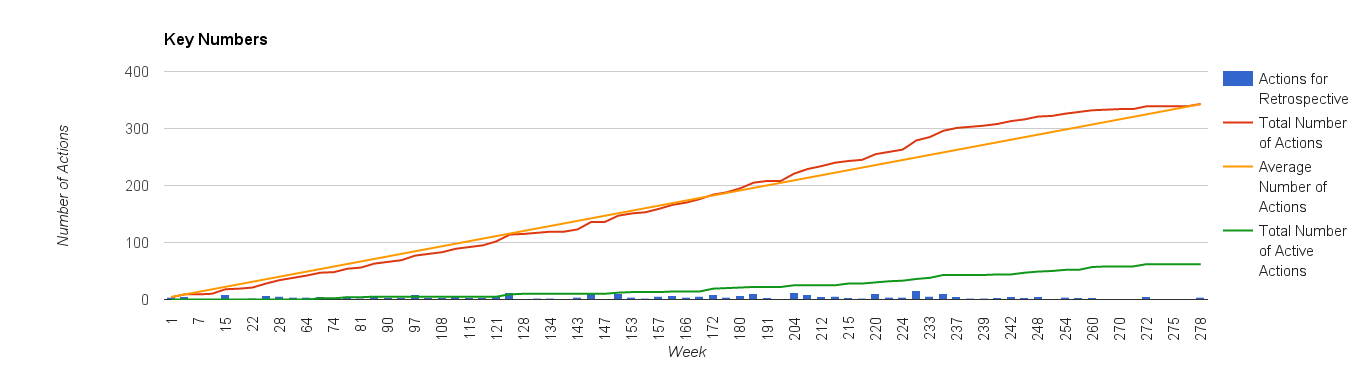
\includegraphics[width=\textwidth, keepaspectratio]{figures/key-numbers.png}
	\caption{A visual representation of some of the key numbers.}
	\label{figure:key-numbers}
\end{figure}
\clearpage	

\subsection{Analysis Results}
In this section we will present the results from our content analysis. We will present the results for each theme defined in \autoref{method:categories}. 

\subsubsection{Nature}
The content analysis revealed that most actions are created as a result of negative problems that has occurred during the development. 89.3\% of the actions were negative, while 5.5\% of the actions were positive and acknowledged good working practices that would be continued. 5.2\% of the actions we lacked the context to determine whether they were positive or negative. As for the distribution of the actions over each retrospective there was no abnormalities except week 97 where there was an unusual amount of positive actions. However while looking into this week we found nothing in particular that could be identified as cause for this spike. As can be seen in \autoref{figure:nature-pa} and \autoref{table:nature-results} the classification of the active actions pretty much mirrored the results from the total actions. 

\begin{table}[!h]
	\begin{center}
	\caption{Analysis results from the content analysis for the nature of the action.}
	\label{table:nature-results}
	\makebox[\textwidth]{%
		\begin{tabular}{| l | l | l | l | l |}
		\hline
		Category & \multicolumn{2}{|c|}{All Actions} & \multicolumn{2}{|c|}{Active Actions}  \\
		\cline{2-5}
		& Number & Percentage & Number & Percentage \\	
		\hline
		Positive & 19 & 5.5\% & 1 & 1.6\% \\
		Negative & 310 & 89.3\% & 57 & 90.5\% \\
		Undefined & 18 & 5.2\% & 5 & 7.9\% \\
		\hline
		\end{tabular}
	}
	\end{center}
\end{table}

\begin{figure}[!h]
	\centering
	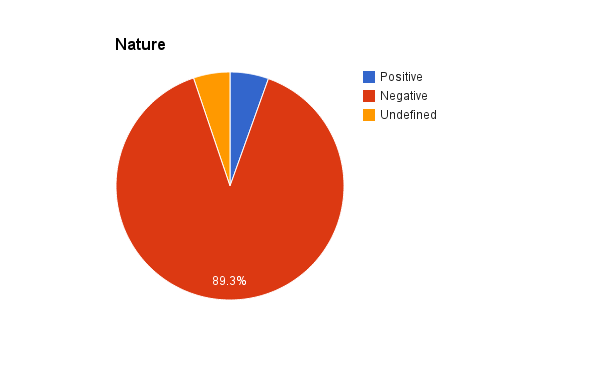
\includegraphics[width=\textwidth, keepaspectratio]{figures/nature-p.png}
	\caption{The negative, positive and undefined distribution of all the actions.}
	\label{figure:nature-p}
\end{figure}

\begin{figure}[!h]
	\centering
	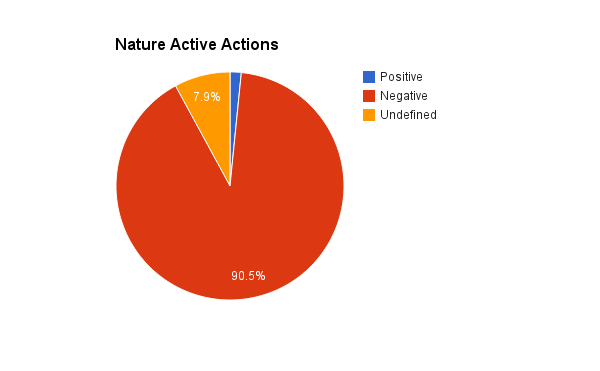
\includegraphics[width=\textwidth, keepaspectratio]{figures/nature-pa.png}
	\caption{The negative, positive and undefined distribution of the active actions.}
	\label{figure:nature-pa}
\end{figure}

\begin{sidewaysfigure}[!h]
	\centering
	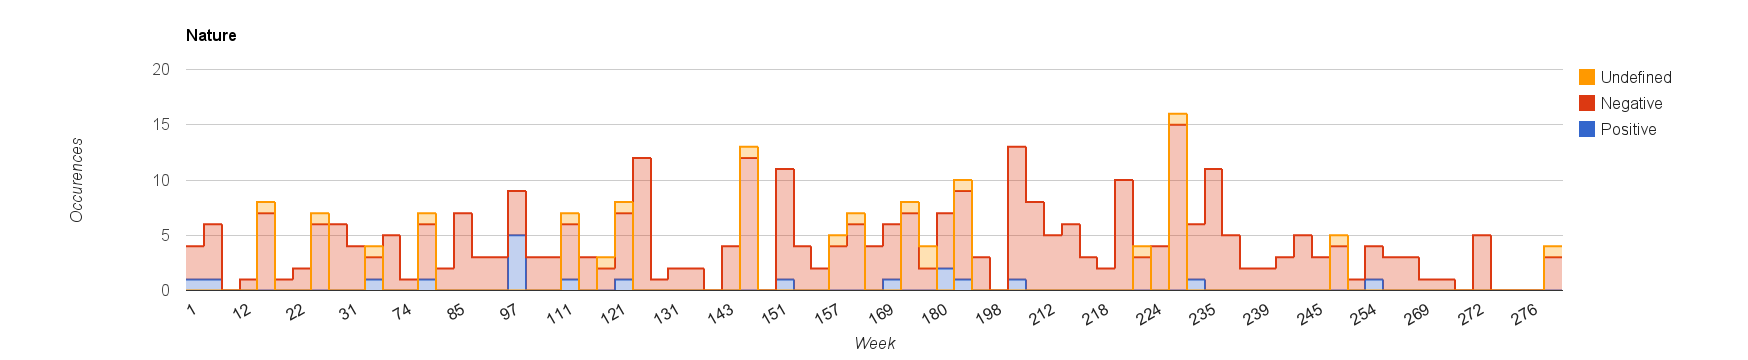
\includegraphics[width=\textwidth, keepaspectratio]{figures/nature-l.png}
	\caption{The distribution of negative, positive and undefined actions across the timespan}
	\label{figure:nature-l}
\end{sidewaysfigure}

\clearpage

\subsubsection{Context}
For the context of the actions analyzed the majority were process related ones. The process actions numbered in 228, which is equal to 58.6\% of all the actions. The Technical ones numbered as 157 which is 40.4\%, while only 4 actions were undefined which results in 1\% of the total actions. As for the distribution over the timespan analyzed there where no abnormalities as can be seen in \autoref{figure:context-l}. For the active actions the results become more equal as seen in \autoref{figure:context-pa}. However it is worth mentioning that the active actions are a sub-group of the total and thus this result is probably a skewed grouping. 

\begin{table}[!h]
	\begin{center}
	\caption{Analysis results from the content analysis for the context of the action.}
	\label{table:context-results}
	\makebox[\textwidth]{%
		\begin{tabular}{| l | l | l | l | l |}
		\hline
		Category & \multicolumn{2}{|c|}{All Actions} & \multicolumn{2}{|c|}{Active Actions}  \\
		\cline{2-5}
		& Number & Percentage & Number & Percentage \\	
		\hline
		Technical & 157 & 40.4\% & 37 & 52.1\% \\
		Process & 228 & 58.6\% & 34 & 47.9\% \\
		Undefined & 4 & 1\% & 0 & 0\% \\
		\hline
		\end{tabular}
	}
	\end{center}
\end{table}

\begin{figure}[!h]
	\centering
	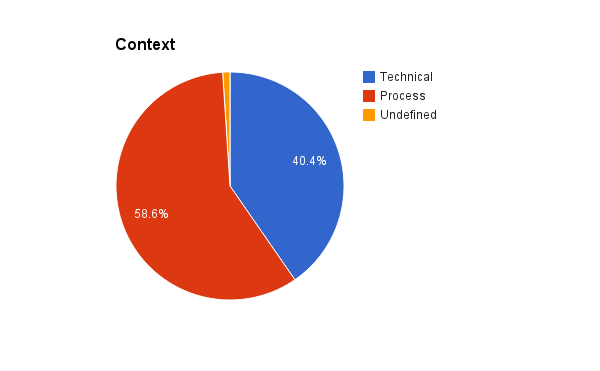
\includegraphics[width=\textwidth, keepaspectratio]{figures/context-p.png}
	\caption{The distribution of technical, process and undefined related actions.}
	\label{figure:context-p}
\end{figure}

\begin{figure}[!h]
	\centering
	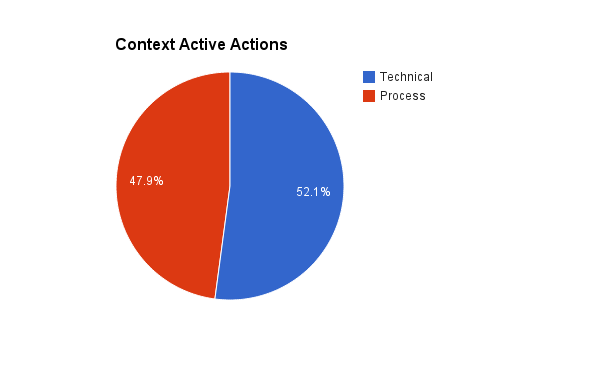
\includegraphics[width=\textwidth, keepaspectratio]{figures/context-pa.png}
	\caption{The distribution of technical, process and undefined related actions over.}
	\label{figure:context-pa}
\end{figure}

\begin{sidewaysfigure}[!h]
	\centering
	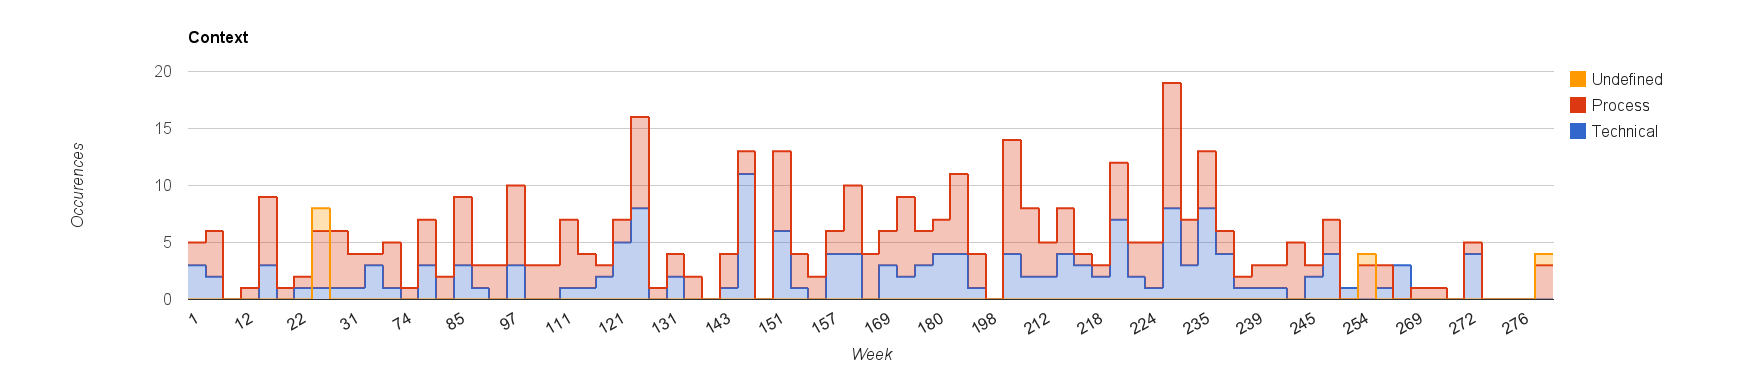
\includegraphics[width=\textwidth, keepaspectratio]{figures/context-l.png}
	\caption{The distribution of technical, process and undefined related actions across the timespan.}
	\label{figure:context-l}
\end{sidewaysfigure}

\clearpage

\subsubsection{Decision Making}
The decision making results showed that the operational decision occurred most in the actions as can be seen in \autoref{table:decision-making-results} and \autoref{figure:decision-p}. Operational decisions occurred in 53.2\% of the actions, while tactical was at 25.9\% and strategic was at 16.1\% of the actions. There only was four cases where we were not able to determine which kinds of decision making type it was. For the distribution over time, as shown in \autoref{figure:decision-l}, there was no emerging patterns and all the decision making types was evenly distributed. The active actions mirrored the total actions almost equal as can be seen in \autoref{figure:decision-p} and \autoref{figure:decision-pa}.

\begin{table}[!h]
	\begin{center}
	\caption{Analysis results from the content analysis for the decision making perspective of the action.}
	\label{table:decision-making-results}
	\makebox[\textwidth]{%
		\begin{tabular}{| l | l | l | l | l |}
		\hline
		Category & \multicolumn{2}{|c|}{All Actions} & \multicolumn{2}{|c|}{Active Actions}  \\
		\cline{2-5}
		& Number & Percentage & Number & Percentage \\	
		\hline
		Strategic & 55 & 16\% & 10 & 16.1\% \\
		Tactical & 89 & 25.9\% & 18 & 29\% \\
		Operational & 195 & 56.9\% & 33 & 53.2\% \\
		Undefined & 4 & 1.2\% & 1 & 1.6\% \\
		\hline
		\end{tabular}
	}
	\end{center}
\end{table}

\begin{figure}[!h]
	\centering
	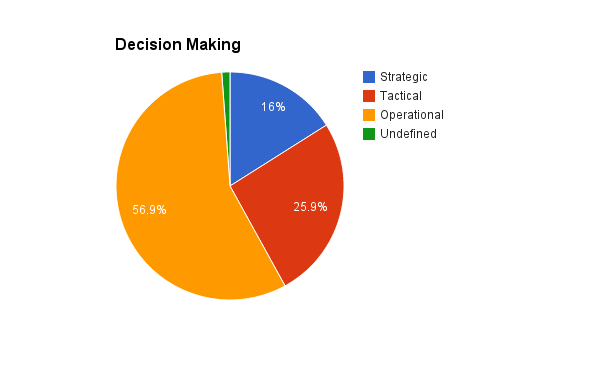
\includegraphics[width=\textwidth, keepaspectratio]{figures/decision-p.png}
	\caption{The distribution of different decision making decisions as they occurred over all the actions.}
	\label{figure:decision-p}
\end{figure}

\begin{figure}[!h]
	\centering
	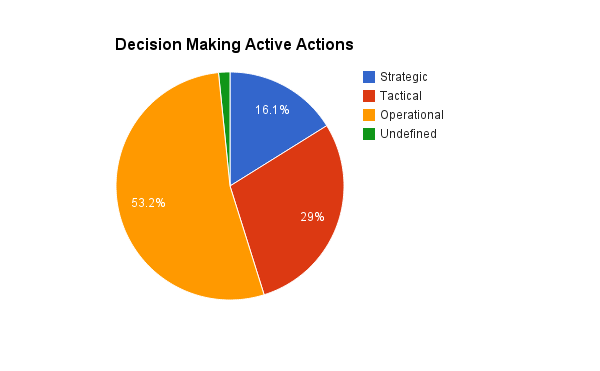
\includegraphics[width=\textwidth, keepaspectratio]{figures/decision-pa.png}
	\caption{The distribution of different decision making decisions as they occurred over the active actions.}
	\label{figure:decision-pa}
\end{figure}

\begin{sidewaysfigure}[!h]
	\centering
	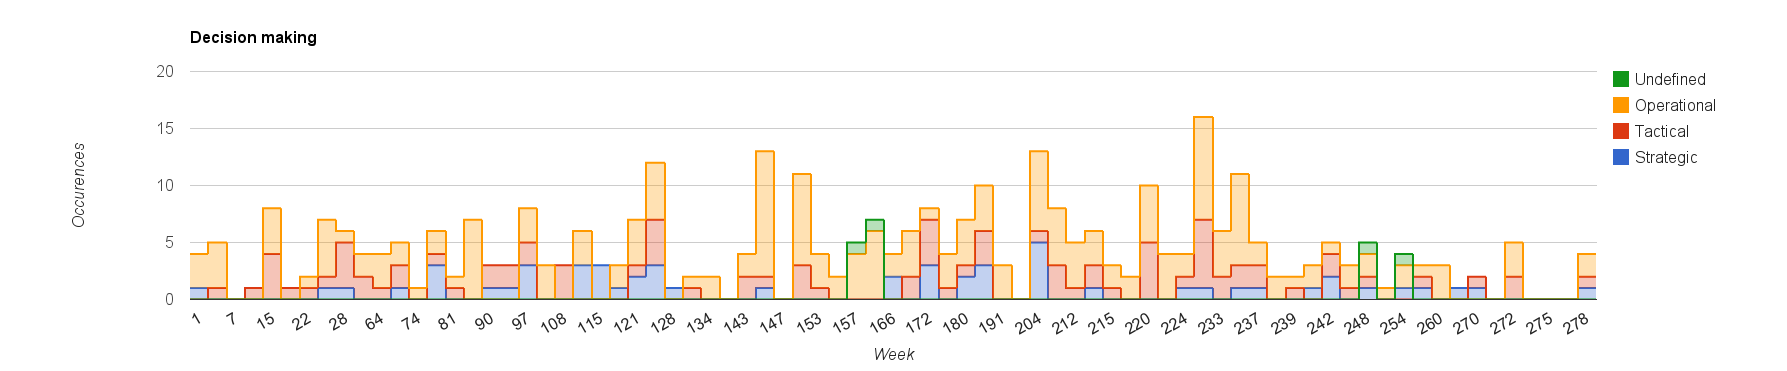
\includegraphics[width=\textwidth, keepaspectratio]{figures/decision-l.png}
	\caption{A timeline showing the distribution of the different decision making decisions for all the actions.}
	\label{figure:decision-l}
\end{sidewaysfigure}
\clearpage

\subsubsection{Organizational Learning}
In terms of organizational learning each action could be defined as single-loop, double-loop or undefined. The results yielded from the content analysis showed that single-loop was the most occurring type of organizational learning with 66.4\% of the actions. Double-loop had 27.2\% of actions, and the rest was undefined at 6.4\%. The distribution over the timespan, \autoref{figure:learning-l} of the analysis showed that the three categories was evenly distributed. The active actions was very similar to the total amount of actions and only had some small negligible variances as can be seen in \autoref{figure:learning-p} and \autoref{figure:learning-pa}.

\begin{table}[!h]
	\begin{center}
	\caption{Results from the content analysis regarding the organizational learning nature of the action.}
	\label{table:organizational-learning-results}
	\makebox[\textwidth]{%
		\begin{tabular}{| l | l | l | l | l |}
		\hline
		Category & \multicolumn{2}{|c|}{All Actions} & \multicolumn{2}{|c|}{Active Actions}  \\
		\cline{2-5}
		& Number & Percentage & Number & Percentage \\	
		\hline
		Single-loop & 227 & 66.4\% & 41 & 66.1\% \\
		Double-loop & 93 & 27.2\% & 16 & 25.8\% \\
		Undefined & 22 & 6.4\% & 5 & 8.1\% \\
		\hline
		\end{tabular}
	}
	\end{center}
\end{table}

\begin{figure}[!h]
	\centering
	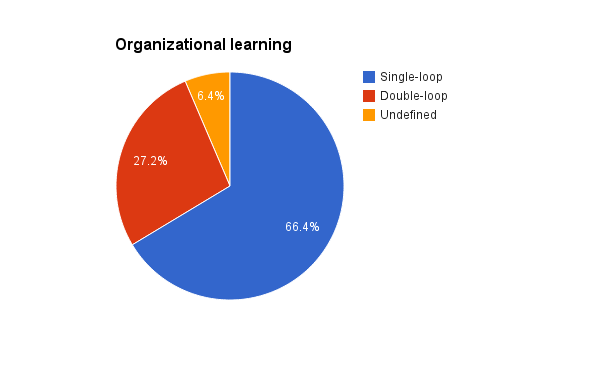
\includegraphics[width=\textwidth, keepaspectratio]{figures/learning-p.png}
	\caption{The distribution of single-loop, double-loop and undefined for all the actions.}
	\label{figure:learning-p}
\end{figure}

\begin{figure}[!h]
	\centering
	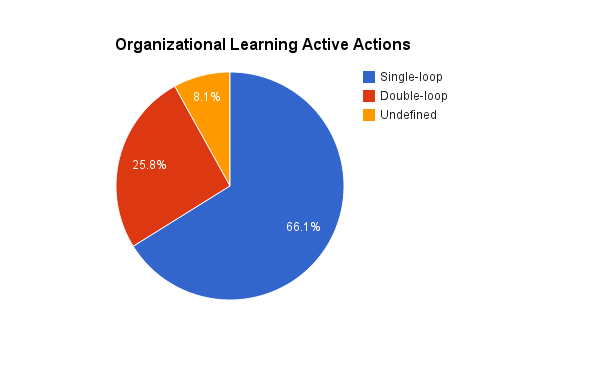
\includegraphics[width=\textwidth, keepaspectratio]{figures/learning-pa.png}
	\caption{The distribution of single-loop, double-loop and undefined for the active actions.}
	\label{figure:learning-pa}
\end{figure}

\begin{sidewaysfigure}[!h]
	\centering
	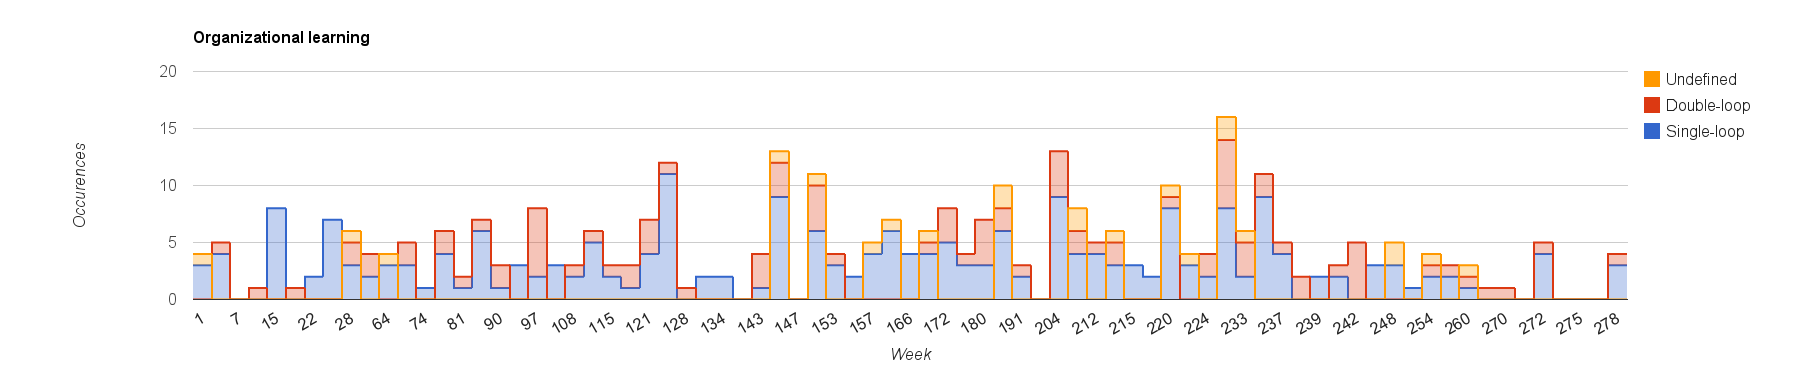
\includegraphics[width=\textwidth, keepaspectratio]{figures/learning-l.png}
	\caption{Timeline showing the distribution of learning loops for the total actions.}
	\label{figure:learning-l}
\end{sidewaysfigure}
\afterpage{\clearpage}

\subsubsection{Development Phase}
Planning, testing, development, and documentation were the four dominant phases in which an action were related according to our content analysis, as can be seen from \autoref{table:development-results} and \autoref{figure:development-p}. Planning being the biggest has a distribution value at 24.6\%. Second is the testing which 21.1\% of all the actions are related to. Development is related to 18.4\% and documentation is 13.2\%. Finally we have the remaining five categories Release, Build, Business Development, Bugfix and undefined which varies between 3.7-6.4 percent as can be seen in \autoref{table:development-results}. 
For the distribution of the different categories over time all of the categories are evenly distributed, in other words; No category is clustered to a specific period in time, but rather occurs evenly through the whole timespan. This can be seen in \autoref{figure:development-l}.
As have been the cases with the other themes the sub-group of the active actions mirrors the total actions with only minor variances as can be seen in \autoref{figure:development-pa} and \autoref{figure:development-p}.

\begin{table}[!h]
	\begin{center}
	\caption{Results from the content analysis in which development phase the action regards.}
	\label{table:development-results}
	\makebox[\textwidth]{%
		\begin{tabular}{| l | l | l | l | l |}
		\hline
		Category & \multicolumn{2}{|c|}{All Actions} & \multicolumn{2}{|c|}{Active Actions}  \\
		\cline{2-5}
		& Number & Percentage & Number & Percentage \\	
		\hline
		Development & 89 & 18.4\% & 11 & 13.1\% \\
		Testing & 102 & 21.1\% & 18 & 21.4\% \\
		Documentation & 64 & 13.2\% & 16 & 19\% \\
		Release & 18 & 3.7\% & 4 & 4.8\% \\
		Build & 23 & 4.8\% & 6 & 7.1\% \\
		Business Development & 18 & 3.7\% & 5 & 6\% \\
		Planning & 119 & 24.6\% & 19 & 22.6\% \\
		Bugfix & 20 & 4.1\% & 2 & 2.4\% \\
		Undefined & 31 & 6.4\% & 3 & 3.6\% \\
		\hline
		\end{tabular}
	}
	\end{center}
\end{table}

\begin{figure}[!h]
	\centering
	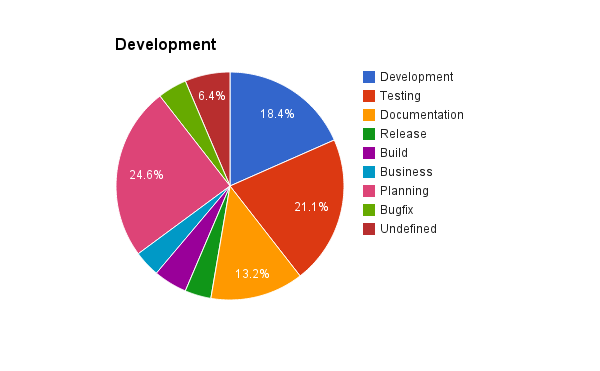
\includegraphics[width=\textwidth, keepaspectratio]{figures/development-p.png}
	\caption{The distribution of the different development phases for all the actions.}
	\label{figure:development-p}
\end{figure}

\begin{figure}[!h]
	\centering
	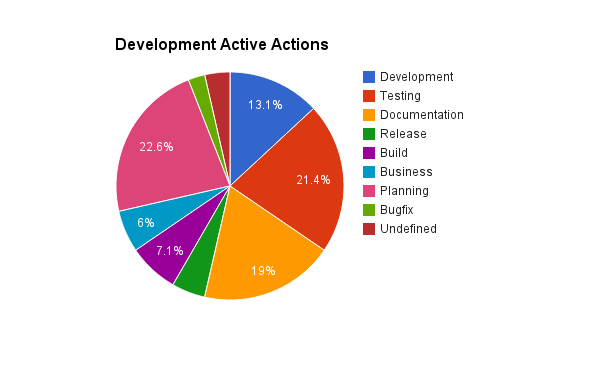
\includegraphics[width=\textwidth, keepaspectratio]{figures/development-pa.png}
	\caption{The distribution of the different development phases for the active actions.}
	\label{figure:development-pa}
\end{figure}

\begin{sidewaysfigure}[!h]
	\centering
	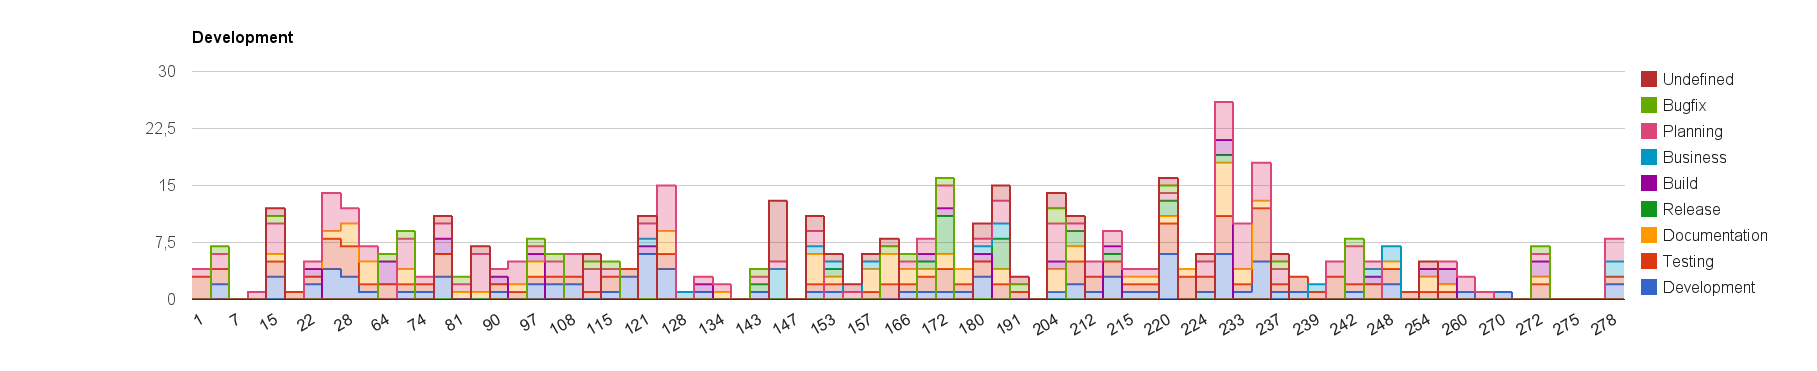
\includegraphics[width=\textwidth, keepaspectratio]{figures/development-l.png}
	\caption{Timeline showing the distribution of the different development phases over time.}
	\label{figure:development-l}
\end{sidewaysfigure}
\clearpage

\subsubsection{Collaboration}
Our results from the content analysis in terms of collaboration showed that 45.3\% of the actions were undefinable in terms of the analysis categorizations we had created. From the actions that were definable Communication was the biggest with 35.2\%. The second was external relations at 11.5\% and third competence at 6.9\%. Finally leadership was the smallest at 1.1\% of the total actions. The statistics can be seen in \autoref{table:collaboration-results} and \autoref{figure:management-p}. 
For the distribution of the different categories over time, \autoref{figure-management-l}, most of the categories was evenly spread across the whole timespan. the only exception to this is week 146 where there is a clear spike of external relations. This spike was a result of the team attending a network meeting in which they did a retrospective to better prepare them for the next network meeting. This anomaly will be disregarded further in the report. 
The active actions, \autoref{figure:management-pa}, shows that the three categories communication, competence and external relations evens out while leadership and undefined remains nearly the same only some small variances. However it is worth mentioning that the active actions are a sub-group of the total and thus this result is probably a skewed grouping. 

\begin{table}[!h]
	\begin{center}
	\caption{Results from the content analysis regarding the collaboration influences of an action.}
	\label{table:collaboration-results}
	\makebox[\textwidth]{%
		\begin{tabular}{| l | l | l | l | l |}
		\hline
		Category & \multicolumn{2}{|c|}{All Actions} & \multicolumn{2}{|c|}{Active Actions}  \\
		\cline{2-5}
		& Number & Percentage & Number & Percentage \\	
		\hline
		Communication & 128 & 35.2\% & 14 & 20.9\% \\
		Leadership & 4 & 1.1\% & 1 & 1.5\% \\
		Competence & 25 & 6.9\% & 1 & 11.9\% \\
		External relations & 42 & 11.5\% & 11 & 16.4\% \\
		Undefined & 185 & 45.3\% & 33 & 48.3\% \\
		\hline
		\end{tabular}
	}
	\end{center}
\end{table}

\begin{figure}[!h]
	\centering
	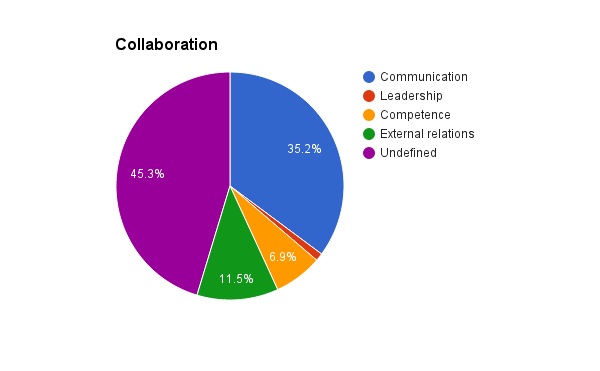
\includegraphics[width=\textwidth, keepaspectratio]{figures/management-p.png}
	\caption{The distribution of different collaboration categories for all the actions.}
	\label{figure:learning-p}
\end{figure}

\begin{figure}[!h]
	\centering
	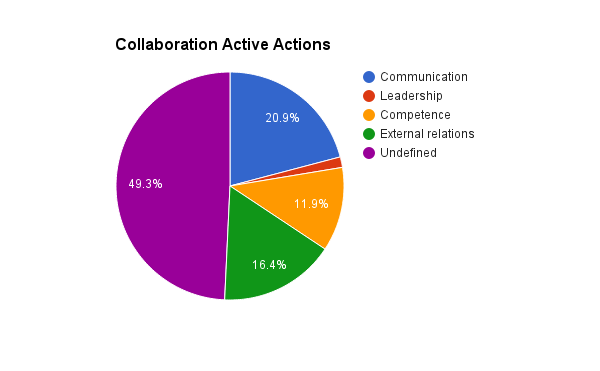
\includegraphics[width=\textwidth, keepaspectratio]{figures/management-pa.png}
	\caption{The distribution of different collaboration categories for the active actions.}
	\label{figure:learning-pa}
\end{figure}

\begin{sidewaysfigure}[!h]
	\centering
	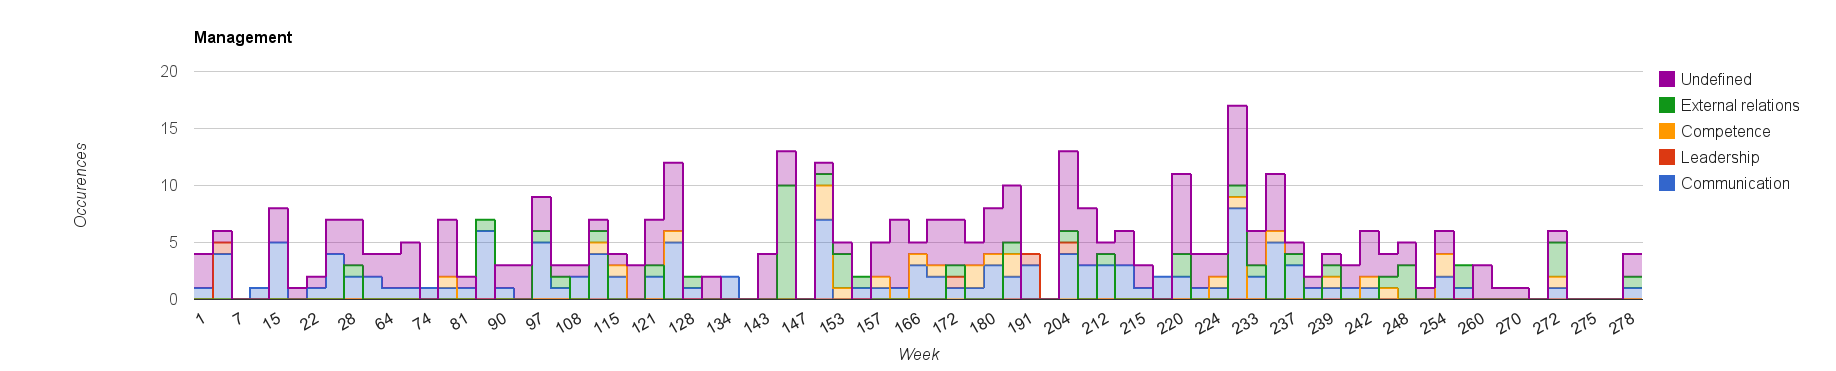
\includegraphics[width=\textwidth, keepaspectratio]{figures/management-l.png}
	\caption{Timeline showing the distribution of the different collaboration categories over time.}
	\label{figure:learning-l}
\end{sidewaysfigure}
\afterpage{\clearpage}

\subsection{Trends}
While conducting our content analysis of all the retrospective actions we uncovered some trends. By trend we mean actions that are related to the same issue/theme. We identified three trends being; Bugfix, Scenario Template and Developer-Tester Communication. We'll go through each of these in the following sub-sections. \todo[inline]{Write about comparing to active actions}

\subsubsection{Bugfix}
The first trend we recognized performing our content analysis was bugfixing. Developing computer systems is sure to create bugs and fixing them then becomes a natural part of developing software. In total we found 20 actions that was related to bugfixing. Of these two were purely technical actions, five were technical and process related and the remaining 13 action were purely process related. Of the 20 actions nine were related to communication between team members. In \autoref{figure:bugfix} one can see that the total amount of bugfixing actions has increased steadily throughout the timespan. 

\begin{figure}[!h]
	\centering
	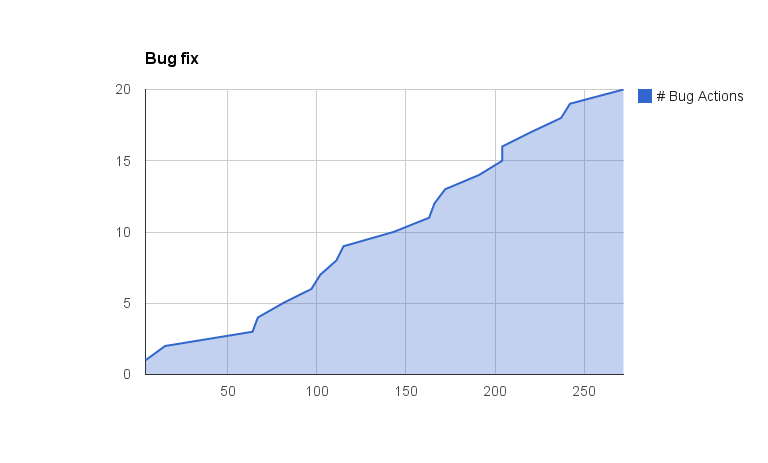
\includegraphics[width=\textwidth, keepaspectratio]{figures/bugfix.png}
	\caption{The total amount of bugfix actions over time.}
	\label{figure:bugfix}
\end{figure}

\subsubsection{Scenario Template}\label{results-ca-scenario-template}
For the second trend we discovered was in relation to a worktool called scenario template that team used to help specify requirements, create user stories and etc. In total we found 25 actions that were related to the scenario template. Of these 25 actions four of the actions were technical and process related, six were purely technical adjustments of the tool and 16 of the actions were process oriented on how the scenario template should be used. 18 of the actions were single-loop, only changing the effects which the scenario template provided. There were also six double-loop actions acknowledging root-cause issues with using the scenario-template and changes to reflect them. 
In \autoref{figure:scenario-template} the total amount of scenario template actions are shown over the 272 week long timespan. One can see that until week 163 the team has a slow increase in the number of scenario template actions. After week 163 however. a huge increase in number of scenario template actions occur. This continues until week 235, with a little slow period between week 180 and 205. At week 235 the team planned a meeting to go through the complete scenario template and after week 235 there are no more actions related to the scenario template. 

\begin{figure}[!h]
	\centering
	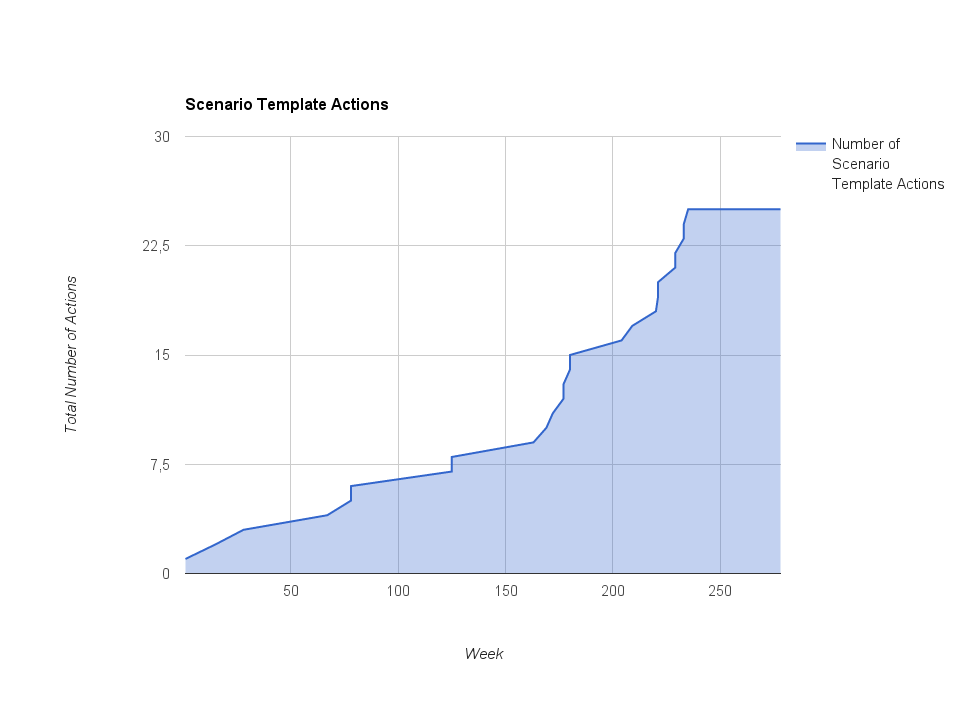
\includegraphics[width=\textwidth, keepaspectratio]{figures/Scenario-tpl.png}
	\caption{The total amount of scenario template actions over time.}
	\label{figure:scenario-template}
\end{figure}

\subsubsection{Developer-Tester Communication}
The final trend we observed during our content analysis was the communication between developers and testers. In total 25 actions were related to this. Of these 24 were process oriented and all the actions occurred from issues with a negative nature. 
\autoref{figure:dev-test-com} shows the distribution of the 25 actions over the 272 week long timespan. It can be seen that for the first 209 weeks that the amount of actions increase slowly with only two to seven actions every 50th week. After week 209 however we see a dramatic increase in the amount of actions, before it completely stops in week 238. We were not able to find any possible reasons for this sudden stop from reading through the reports. However as can be seen from \autoref{figure:dev-test-com} there has been periods between actions as long as 45 weeks so it is possible that this stop can be such a break.  

\begin{figure}[!h]
	\centering
	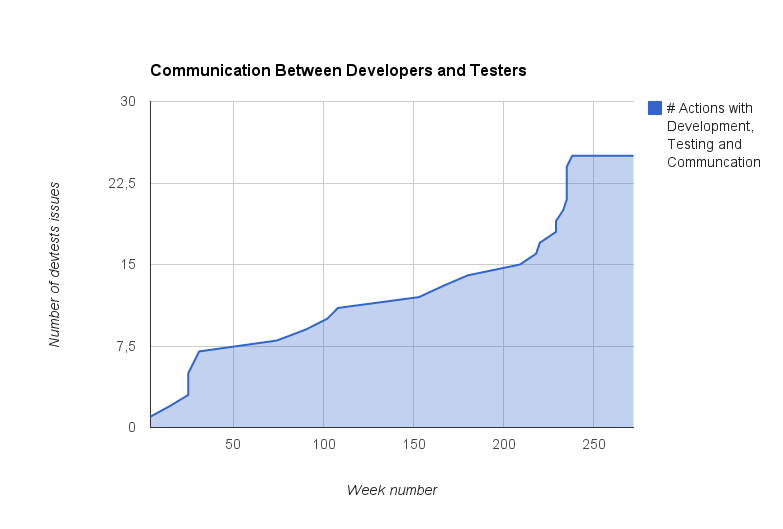
\includegraphics[width=\textwidth, keepaspectratio]{figures/devtestcom.png}
	\caption{The total amount of developer-tester communication related actions shown over time.}
	\label{figure:dev-test-com}
\end{figure}

\clearpage

\section{Feedback Session}
After performing our content analysis, we visited the team to present our analysis results as well as receive feedback from the team. In this section and its following sub-sections we'll present the results from this session. We will start with going through the feedback on the key numbers, before we continue on the categories and trends and finally take anything else that came up during the session. 

\subsection{Feedback: Key-Numbers}
When presenting the key-numbers the team mostly found our results agreeable with their own thoughts. The only surprise to the team was the amount of active actions. Their surprise came as they believed the number of active actions to be higher. The reason for this belief was that they thought they were worse at closing actions as the list of active actions seemed so long, but compared to the amount of total actions it seemed more reasonable. However it was pointed out that existing actions hinder new actions for the same problem to be created and thus the amount of active actions might not be accurate with how the team works with the problems as a actions might not be documented, but worked on never the less. 

\label{results-elephant-in-the-room} When raised the question why the decrease of actions after week 237 the team gave their thoughts. During the period the decrease in number of actions they had acquired a new foreign developer within the team. Unfortunately the new developer had not lived up to the task creating what the team called an ``Elephant in the room''.\todo[inline]{Del dette opp i to setninger} The situation absorbed the other problems within the team as no one would be rude and tell that the new developer that he were the problem. As one of the team members described during the feedback session: 
\begin{quote}
``We actually discussed it once at the coffee after lunch, the retrospectives at the moment were just a waste of time''. 
\end{quote}
When asked what was the reason for the developer not living up to his expectations the team told us that face-saving and cultural differences made it difficult to communicate properly and that tasks that were assigned to him weren't satisfiable. 

The developer quit the team after a period of 34 weeks in week 263. This still means that the low action period of 15 weeks between and week 263 and 278 remained unexplained. When inquired about this the team had several possible reasons. One were that there were already to many active actions on the plate resulting in fewer getting made. Another were that the communication within the team improved after team had lost the developer creating the problems. A final possible reason was that the secretary for the retrospectives changed a lot within that period of time. 

After discussing the decrease in actions period the team mentioned that it would be interesting to see if there were any correlations between retrospective actions and team changes other than the one already explained. We have in the time after the visit to the team created such charts as can be seen in \autoref{figure:team-changes} and \autoref{figure:secretary-changes}. 

In \autoref{figure:team-changes} we can see that the period of low actions starting at week 237 and lasting out week 278. In that period the foreign developer, T7, joins and leaves the team. In the same period the SCRUM master of the team takes a leave of absence for a period of 20 weeks which also might have influenced the period. 

For the secretary changes, shown in \autoref{figure:secretary-changes} we can see that the changes in who writes the reports doesn't seem to influence the number of actions that comes out of the actions. The only exception to this could be the period after week 263 where there are a lot of changes, as the team described. However we believe this to be unlikely as between week 270 and 275 the secretary stays the same and the amount of actions follows the trend of low number of actions and as changes earlier in the timespan haven't revealed any effects. 

\begin{sidewaysfigure}[!h]
	\centering
	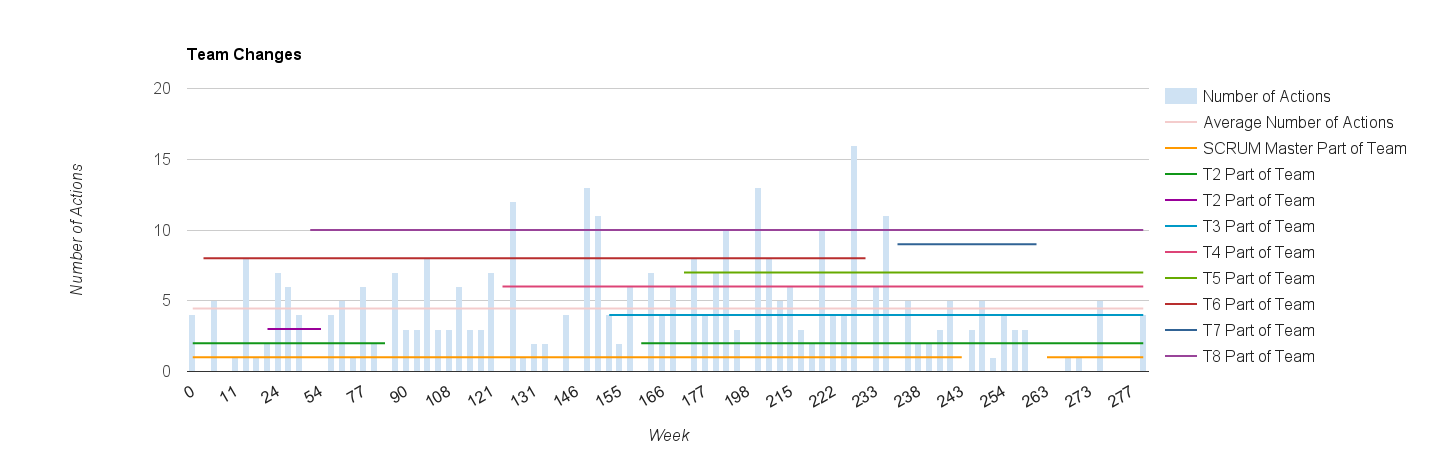
\includegraphics[width=\textwidth, keepaspectratio]{figures/team-changes.png}
	\caption{Team changes and the amount of actions for the retrospectives across the 278 Weeks.}
	\label{figure:team-changes}
\end{sidewaysfigure}

\begin{sidewaysfigure}[!h]
	\centering
	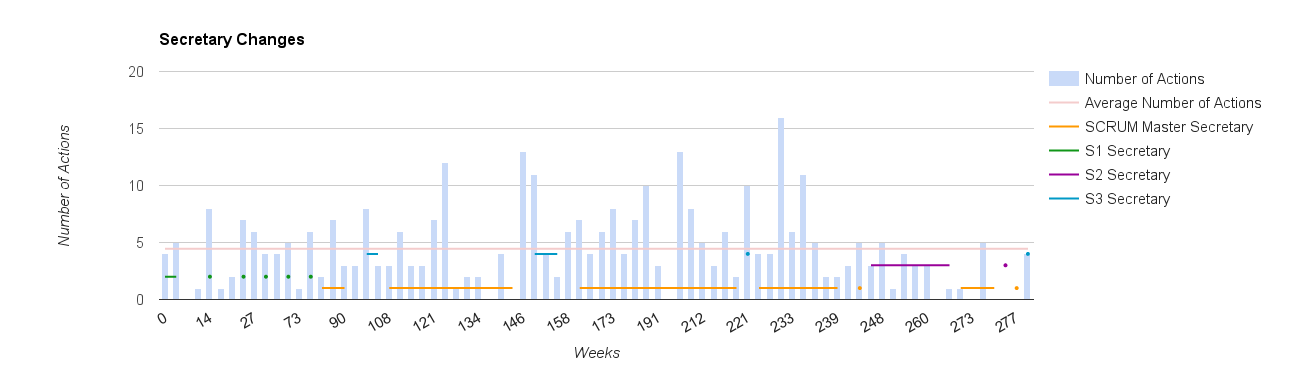
\includegraphics[width=\textwidth, keepaspectratio]{figures/secretary-changes.png}
	\caption{Secretary changes and the amount of actions for the retrospectives across the 278 Weeks.}
	\label{figure:secretary-changes}
\end{sidewaysfigure}
\afterpage{\clearpage}

\subsection{Feedback: Categories and Trends}
In this section we will present the thoughts of the team as well as their reactions on the results of the content analysis. We will start with the nature of the actions and then continue on context, decision making, organizational learning and development phase and finally we will go through the collaboration categories and trends. 

\subsubsection{Nature}
The results from the nature context did not surprise the team at all. We asked if they would like the guess what the ratio between positive negative would be and they said one-to-nine, which is quite close. Our results revealed five percent undefined and five percent positive with the remaining 90 percent negative. The team described themselves as problem-oriented and reasoned that this is the cause for the high amount of negative actions. They also said that they do during the retrospectives talk about good things that has happened, but as they are problem oriented it rarely gets documented. 

\subsubsection{Context}
Our results from the content analysis revealed that 58 percent came from a process context, while 40 percent came from a technical context. When this was presented to the team they thought it would be more technical than process actions. The reason for this wasn't elaborated during the session. It was however elaborated on the results of the active actions which the analysis revealed had a little more technical actions than process ones. The team said this was not so surprising as some of the technical actions could require a lot of time to complete. 

\subsubsection{Decision Making}
The team thought that it was a good sign that the team were able to do strategic decision making. When we presented the results for the decision making analysis, the team was pleased to see that they had all of the three categories represented. They were especially pleased to see that the there was a substantial portion of strategic actions. We asked what could be the reason for this and the team responded that they felt autonomous. As they described the company allowed the different development teams to have a fairly large independence allowing room to do strategic choices within the team. 

\subsubsection{Organizational learning}
When we presented the team to our results in terms of organizational learning the assumptions they had was as expected. They use the term of direct causes as single-loop and root causes as double-loop, but we will continue using the terms of single-loop and double-loop. They expected that single-loop would have the most occurrences, even though they maintained a double-loop focus during the retrospectives. This expectation is reflects our results quite well as 66 percent were single-loop and 25 percent double-loop. The reason they expected it to be more single-loop rather than double-loop was that it was easier to do single-loop and as one team member said: ``...sometimes things just need to be fixed''. 

\subsubsection{Development Phase}
The results from the content analysis were quite different from the team expectation in the context of which development phase the actions were related. The team expected that build and documentation would be the two biggest actions. The content analysis revealed that planning was the biggest followed by testing, development and documentation. The team thought this made sense as most of the planning is directed towards process improvement and they do focus on process during the retrospective. The team speculated if the releases might have a correlations with planning actions coming right after. It was also again mentioned that actions might not be created even though they were discussed as actions already existed and that they had not been completed. 

The team expected build to be the phase that occurred most. It was a surprise that it was not better represented within the actions as it felt that it was discussed often on retrospectives. One of the members said that the lack of actions specific for builds might be the reason while it was discussed during retrospectives and that they might focus on creating more actions related to the builds. 

We asked the team if there were any categories they missed from the development phase analysis and two were mentioned. The first one was hotfix which the team often mentioned during the feedback session. The second one was flow as to how the development of the product progressed. For future similar analyses this should be taken into considerations. 

After the visit to the team we took the time to create a chart showing releases against the number of actions and planning actions as displayed in \autoref{figure:releases-and-planning}. These results provided intersting data. As can be seen in \autoref{figure:releases-and-planning} the releases does not have any impact on either the amount of the planning actions or number of actions in total. This is interesting as the team themselves expected there to be a correlation and reasoning thoughts would have expected the same. 

\begin{sidewaysfigure}[!h]
	\centering
	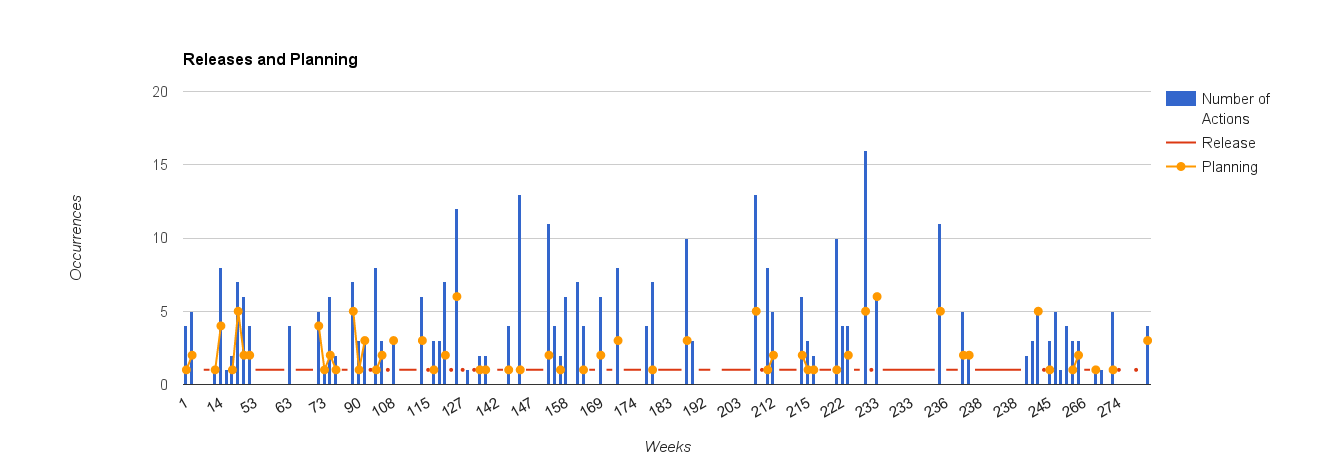
\includegraphics[width=\textwidth, keepaspectratio]{figures/releases-and-planning.png}
	\caption{Correlation between release and planning actions}
	\label{figure:releases-and-planning}
\end{sidewaysfigure}
\afterpage{\clearpage}

\subsubsection{Collaboration}
For the collaboration the team expected communication to be the category with the most actions. If you disregard the undefined actions which was the biggest in terms of collaboration the teams expectation was correct. We asked if they could explain what kind of communication that were discussed most during the retrospectives. They said that communication between the different stages of the development and more oral communication rather than written was the kinds of communications that were discussed the most. As for the other categories the team had no special feedback.

\subsubsection{Trend: Bugfix}
When we presented the bugfix trend to the team they were surprised that we had identified it as a trend. The surprise came as a result that they had found a way to work with the bugs. Having dedicated bug-days was a practice that had been implemented and used for the last year which the team found very helpful. As can been seen from \autoref{figure:bugfix} the amount of actions still continue to increase after the implementation of the bug-day. When inquired by this the team told us that even though the bug-day worked very well, they still wanted to improve and that was why the actions still was increasing. 

\subsubsection{Trend: Scenario Template}
The trend of scenario template changes provided surprises both for the team and the researchers. As described in \autoref{results-ca-scenario-template} the retrospective reports indicated that during week 235 a meeting were scheduled to go through the whole template. After this action no more actions occurred during the timespan. The researchers expected it to be a classic case of taking the root-cause, double-loop learning and the problem disappeared. However the scheduled meeting were never held. The team discussed several reasons for why this could be the case. One were that they still might be waiting to hold that meeting. Another was that a cleanup had been done, and changes to the scenario template still occurred, but that actions on it were not created. A third possibility was that the same period they had a team member that didn't work out as described in \autoref{results-elephant-in-the-room}. Unfortunately the discussion ended only with possibilities and no conclusion. 

\subsubsection{Trend: Developer-Tester Communication}
The final trend, developer and tester communication returned similar feedback as the scenario template trend. The pattern identified in the content analysis where after week 238 the actions related to developer tester communication stopped. The team again found several possible solutions. The first one was, as mentioned in \autoref{results-elephant-in-the-room}, the team member which did not fit the team. Another possible reason was the secretary changes as well as the scrum masters leave of absence. The team also said that most of the communication had been mostly oral and handover meetings had been introduced and that this worked pretty well. The team seemed to believe that all the mentioned reasons would explain the stop of developer-tester communication actions. 

\subsection{Other Feedback From the Feedback Session}
Several other things were mentioned by the team during the feedback session. 

The team found the presentation and analysis very useful. It was described as a refresh on retrospectives and they speculated if it was possible to develop a tool that could codify the actions from a retrospective and visualize them on a dashboard. They found the presentation provided a good awareness on the retrospectives, which earlier had not been that good. They also decided that they should focus more on finding root-causes as the presentation gave a short introduction to single-loop and double-loop learning.

It was also mentioned that only the actions doesn't necessary reflect the complete retrospective meeting. Good things are usually not created to actions as may other things be. 
\clearpage

\section{Feedback interview}
The interview lasted for almost 1 hour, and was recorded and transcribed. At the start of the interview we did a short recap of the presentation. During this recap the interviewee expressed satisfaction with the analysis, and agreed with the constructed framework for analysis. The interview revolved around three main subjects that were discussed, team dynamics, organizational learning and retrospectives.
\todo[inline]{Generally make sure that all the blue post it notes are reflected in the text.} 
\subsubsection{Team dynamics}
\todo[inline]{bygg ut denne paragrafen litt.}
During the interview the scrum master spoke about how he considered his team mature and willing to learn. Over time the team had developed an ownership feeling regarding the retrospective, and that this had been developed through working with it over time. Another important element was that a high degree of trust between team members led to productive session. An important part of this is that every team member feels that they are taken seriously.

\paragraph{Cultural differences}
He also elaborated on how cultural differences could impact the tone of retrospectives. One example was a new team member from a different country leading to communication problems. The team member was concerned with losing face and therefore did not communicate problems with the rest of the team. These communication problems became so prevalent that that they directly influenced retrospectives. Team members would consider the communication problems so major that they would consider more minor, and fixable issues irrelevant, thus leading to little or no issues being solved at all.  Other team members described this situation as an ``Elephant in the room'' that overshadowed all other issues. This was not handled in the retrospective since personnel issues were not considered within the domain of the retrospective.

\subsubsection{Organizational Learning}
\todo[inline]{Oppf;lgings paragraf kan kanskje flyttes hit?}
On the subject of organizational learning the interview discussed how a team learns and how it relates to the the retrospective. An interest was expressed in doing a more comprehensive analysis of the retrospectives within the team, but a major concern was a possible waste of time, with little return on investment. One example mentioned by the interviewee was the arrangement of a ``bug-crunch'' day that was created during the retrospective lead by the external facilitator. The ``bug-crunch'' day is a day set aside solely to the elimination of bugs and similar issues, the day is held at regular intervals. This was described as a very positive change that had led to a clear decline in bugs. When discussing the process of spreading the lessons learned within the team to the outside there was no clear process for this, but creating a ``notable efforts'' documentation where positive efforts were documented was considered. 

\subsubsection{Retrospectives}
The current state of the retrospective in the team was described as a simple meeting where team members could speak their mind and discuss any issues they themselves wanted to bring up. However they had experimented with some different retrospective techniques and found them interesting, and considered using them occasionally. An important part of the retrospective was an attempt to reach a consensus. The tone of the retrospective was described as light, but sometimes could get more heated during discussions. The retrospectives were held every 3rd week, but could sometimes be moved due to pressure related to releases or other pressing issues
When asked about how the team members prepared for a retrospective he commented that there was a variety of approaches, some team members made lists beforehand and arrived prepared, while others were more impulsive and decided on their issues during the retrospective. . 

\todo[inline]{Egen paragraf for hvert nye tema. Denne for eksempel er en lederskaps paragraf}
The use of external facilitators was an interesting concept, and the one experience they had with using one had been a positive experience.\todo[inline]{SCrum master not feeling like a leader but a facilitator. Also leader particpating makes it easier to take strategic decisions}

\paragraph{Task follow up}
He described the current action assignment as ``push'' based where an issue was delegated to a team member, often the one with expertise relevant to the issue. Also mentioned was a desire to introduce a more ``pull'' based system where tasks could be chosen by team members at their leisure. A major issue was the problem of enforcing a process related, as there existed no formal tool or process for ensuring that the process actions were actually employed. A lot of the actions were quick fixes that were handled rapidly by whoever were delegated the task.
\clearpage

\section{Feedback Interview 2 Results}
\label{second-feedback-results}
The start of the second feedback session revolved around discussing event analysis, where the amount of actions were plotted next to events like staff change or secretary changes. \todo[inline]{Legg til litt om denne graf analysen? Eller link?} The session revealed two major changes after our first analysis, as well as a process change. The first major change that was mentioned was that the focus of the retrospective had become more positive, with participants making sure to bring up positive issues. This change was considered an improvement by the team leader. A second change was a different attitude in the team towards the unresolved retrospective actions. \todo[inline]{Legg til ett direkte sitat? Transkiber den delen.} The previous attitude was to think of the list of unresolved actions as a great mass that just grew, with little appreciation for the large number of actions and improvements were accomplished. The team leader expressed that this had led to a more positive environment. The team also planned to include retrospective actions in a maintenance day that was held at regular day, in order to make sure that resources were delegated to solving the actions. 

\clearpage
\section{Interview Results}
In this section, and its following subsections, we will present our results from the semi-structured interviews. We will present the results in relation to the different themes discussed during the interview: ``General'', ``Organizational Learning'', ``Team Dynamics'', ``Team specific'' and ``Anything Else''. We will not present every statement made by all the interviewees, but focus on the unique results that came out of the interviews. 

\subsection{General} % (fold)
\label{sub:general}
\todo[inline]{Create some tables for characteristic questions or responses and how many team that said the same}\

All participants we interviewed worked as a part of a team, we asked everyone to describe their team in order to gain insight in the circumstances surrounding the retrospective.  One of the teams, team Echo, was large with ten people working on several different products at the same time. The team was then divided in the subject where members worked on one or more products, this led to a small amount of infighting and divisions. The retrospectives were also affected as not everyone had the same experiences or problems. This led to time being wasted for team members as issues beyond their scope were discussed in plenum. In team Alfa and team Foxtrot this was not mentioned as a problem. 

Team Charlie was a small team of four developers, where all were highly experienced, with especially two of the developers holding very senior positions within the company. The two senior developers were described as especially strong personalities. The team was described as very eager to learn and always searching for ways and ideas that could be used to improve the team. The strong personalities influenced the retrospectives in that sometimes the junior developers would agree without arguing strongly for their own ideas or suggestions. Another interview participant from team Delta also described his team as very eager and they considered the retrospective meetings the most important process during development. 

\label{question-3}
When we asked the different developers and SCRUM masters how they conducted the retrospectives we got a wide range of answers. 

Team Echo started their retrospective with ranging on the range one-to-nine the three categories team flow, team moral and technical quality. This allowed them to see trends on the three categories. When we asked what happened if something was graded really low the response was that it had not happened yet. We also asked if the opposite what happened if something was graded really high and the response was the same that it had not happened yet. After the grading the team used KJ-sessions, where one write positive and negative issues on post-it notes and then discuss them in the group. Which Dingsøyr et al. describes as a structured brainstorming technique \cite{Dingsoyr2003}. According to the developer the things that came up during the KJ-session was really specific things related to the work environment. The reason for this was that the team worked on different pieces of software and that each sub-team had their own process. 

Two of the teams, Charlie and Echo, varied each time how they conducted the retrospectives. The reasons for this was to challenge the comfort zone of the members as well as counter group thinking and monotone activities. Group thinking is the desire for cohesion in a team and McAvoy and Butler \cite{Mcavoy2007} refers to it being considered as way to ineffective decision-making. 

We asked the SCRUM master in team Delta if it always was new techniques or if some were repeated. The response was that the same technique never came twice in a row, but techniques that worked well would be repeated on several retrospectives. As to how they found the new techniques they used several sources. Blogs, websites like retromat \cite{Retromat2015} and agile podcasts were all mentioned as a good way of obtaining new techniques. 

During our discussion we asked if there were any downsides to use such varying techniques. Team Charlie's SCRUM master said that the for some participants it could become a little bit too much. This could result in lower enthusiasm for the retrospective. \todo{Lytte igjennom intervjuet med espen, hvor mye var for mye. }. Another downside was that for some techniques the focus could move to the technique instead of the issues which could lower the results of the retrospective. However he said that he still found that varying the retrospective techniques was beneficial to the retrospective. \todo{Lytt igjen fil med stian og h;re hva syntes}.

\todo[inline]{Team alfa and varying depending on feature or workprocess retro}

\begin{table}[!h]
	\begin{center}
	\caption{Retrospective Techniques Used}
	\label{table:retrospective-techique}
	\makebox[\textwidth]{%
		\begin{tabular}{ l  l }
			\hline
			Team & Technique \\
			\hline
			Echo, Alfa, Foxtrot & KJ-session \\
			Zulu & Team Discussion \\
			Alfa, Charlie, Delta & Varying Techniques \\
			Echo & Team Barometer \\
			Foxtrot & Weather Forecast \\
			\hline
		\end{tabular}
	}
	\end{center}
\end{table}

\label{question-3a}\todo{Update as we get more information}
The duration and frequency varied between the different interview participants. An overview can be seen in \autoref{table:frequency-duration} One team held retrospectives every week, while another team held every second week and yet another team held every third week. The SCRUM master for the team that held the retrospective every week said that doing it every week gave continuously follow-up. The team regarded the retrospective as the most important meeting during the development and all the team members saw the value that the retrospective provided. 

One of the teams we spoke to performed retrospectives at irregular frequency. Instead of conducting retrospective after each sprint or at a given time they performed retrospectives after they had finished each major feature in their project. They also conducted retrospectives whenever one person in the team felt it was necessary. Usually a retrospective were held once a month. This resulted in two kinds of retrospectives being conducted. One feature retrospectives where persons actively working on that feature participated and the complete development process of that feature was discussed. And one work process retrospective which handled general work processes for the team. This latter retrospective was conducted by an external facilitator. Of the two retrospectives the feature retrospective was the most common. 

We interviewed two members of this team, one developer and the project leader. Both the developer and project leader found that feature driven retrospectives worked very well. However the developer admitted that he sometimes missed having all members of the team participating in the retrospective. Currently only the people actively participating in the development of the feature was invited to the retrospective. The developer said that there was a risk that some members of the team might participate in a retrospective rarely as their assignments didn't necessarily resulting in a feature being created. 

\label{question-3b}\todo{Update as we get more information}
The duration of the retrospectives varied between the teams, from a fixed amount of hours to until ``we are done''. For those having fixed time one team had 1 hour, while another had 2 hours long retrospective. 
\begin{table}[!h]
	\begin{center}
	\caption{Frequency and duration for the different teams}
	\label{table:frequency-duration}
	\makebox[\textwidth]{%
		\begin{tabular}{ l | l | l }
		Team & Frequency & Duration \\	
		\hline
		Delta & Every week & 1 hour \\
		Charlie, Echo & End of every sprint & 1-2 hours \\
		Foxtrot & Every second week up to six months & 0.5-4 hours \\
		Alfa & End of every released feature & 1-2 hours \\
		Alfa & On request by team member & 1-2 hours \\
		\hline
		\end{tabular}
	}
	\end{center}
\end{table}

\label{question-8}

\label{question-6}
The steps taken to enforce actions created during the retrospective and whether unresolved actions was a problem varied between the interviewed teams. 

One team used several techniques. Some actions were added to the sprint backlog as it helped reminding the team that it needed to be done. The actions that were related to the work environment was usually handled by the SCRUM master. Reaching a common consensus was something that the team regarded as a beneficial way of getting things done. Finally the team, along with other interviewed teams, always assigned a name to the actions found during the retrospective. This ensured that a person would have a responsibility to the action and at every retrospective the team would take a quick round to see if the action had been completed. We asked the developer what happened if someone forgot to do it and he replied that it was noticed by the other members of the team and it had never occurred that an action had been unresolved over two retrospectives. This resulted in that most actions become resolved as was the case with other teams that assigned names to the actions. \todo{Confirm statement when all results are in}. One of the other teams that assigned names to the actions said that most actions were resolved however new routines that were part of an action that were not working would not be done regardless of names assigned. These new routines however was later deemed bad routines as it did not work when it was practiced. 

A team managed to resolve most of the actions created. They assigned names to the different actions and the project leader said this was more effective rather than not doing it, which they had done earlier. Some actions however the team wasn't able to resolve. There were several reasons for this. Some of the actions became really creative and thus was difficult to implement. Other actions was huge and required resources the team didn't have. 

Follow-up by the SCRUM master of the team was generally regarded as an important measure to help resolved actions from the retrospective by several teams. Also adding the actions to a SCRUM board or a separate board was regarded as a good measure to get actions resolved. 

One of the SCRUM masters admitted that very few of the actions they created was resolved. He told us that actions were not assigned to individuals, but rather the group as a whole. As part of the leadership for the department he had participated in a retrospective for the department as a whole, where individuals had been assigned to different action. This had not worked in that retrospective and thus he was hesitant to do this in his own team. We asked if unresolved actions created a negative loop, where enthusiasm for the retrospective went down as improvements never came and the low enthusiasm made sure fewer actions were resolved. His reply was yes, it did create a negative loop, which needed to be countered. He also hoped that having a whiteboard to put the actions up on would help remind the team to resolve some of the actions. 


\begin{table}[!h]
	\begin{center}
	\caption{Action Follow-Up Techniques Used}
	\label{table:follow-up-techique}
	\makebox[\textwidth]{%
		\begin{tabular}{ l | l | l }
		Team & Follow-up technique & Satisfied \\	
		\hline
		Echo, Delta, Alfa, Foxtrot & Assigning Name to action & Yes \\
		Charlie & Assigning to group & No \\
		Foxtrot & Adding to backlog & No \\
		Delta & Visualizes Action & Yes \\
		Echo & Handled by SCRUM-master & Yes \\
		\hline
		\end{tabular}
	}
	\end{center}
\end{table}
 
\label{question-7}
One SCRUM-master said that personality might hinder the function of the retrospective. In his department SCRUM masters had been assigned to developers in teams where generally only was developers. This had for some of the teams become a problem. In those teams that the enthusiasm lacked within the SCRUM master as they rather would just do regular developing and this could spread to other team members as well. 

In another team, a developer told us that the one hinder for getting value from the retrospective was too long timespan between the retrospectives. In that team retrospective could be held on irregular times ranging from two weeks up to six months. If the timespan was to big, the retrospective returned no value as there simply was to much too discuss according to the developer. 

\begin{table}[!h]
	\begin{center}
	\caption{Value Decreasing Hinders for the Retrospective}
	\label{table:value-decreasing-hinders}
	\makebox[\textwidth]{%
		\begin{tabular}{ l | l | p{0.5\textwidth} }
		Team & Hinder & Description \\	
		\hline
		Charlie & Personality & SCRUM-masters who is not motivated to do retrospective creates low enthusiasm in the group. \\
		Foxtrot & Timespan between retrospectives &  Having too long time-spans between retrospectives creates more topics which takes longer to discuss and thus is unproductive. \\
		\hline
		\end{tabular}
	}
	\end{center}
\end{table}

\label{question-9}
Encouraging learning with external things like bonuses and such was not used by any teams. The closest was one team that had sometimes brought some pastries to the meeting. One developer said that encouraging through bonuses would be a destructive force in the retrospective and the focus would be removed from the process.

\label{question-10}
There were different views on facilitating retrospectives. Several team used an external facilitator and said that they would encourage others to do the same. The benefits was that the external facilitator was able to see things that existed within the team, that the team themselves were not aware of. The external facilitator was not hired as a facilitator, but rather a SCRUM master from another development team.

Other teams had not been using external facilitators. They used their regular SCRUM master. Common for the SCRUM masters were that they all felt like they were a facilitator rather than a leader during the retrospectives. Those we spoke to about external facilitators were positive to the idea and mentioned they might want to try it out in the future. 

\begin{table}[!h]
	\begin{center}
	\caption{Usage of external facilitator}
	\label{table:external-facilitator}
	\makebox[\textwidth]{%
		\begin{tabular}{ l | p{0.3\textwidth}}
			External facilitator & Teams \\
			\hline
			Used external facilitator & Alfa, Echo \\
			No external facilitator & Charlie, Delta, Foxtrot \\
		\end{tabular}
	}
	\end{center}
\end{table}
% subsection general (end)

\subsection{Organizational Learning} % (fold)
\label{sub:organizational_learning}
The different teams learned in different ways during the retrospective.

\label{question-11}
To create a common ground for discussing organizational learning we asked if there was any specific things that had changed in how the team worked or thought, through the retrospective. One team had for a while been using much time on estimating the time needed to complete a user story. The estimations turned out to be generally wrong and during a retrospective this had become a discussion. This resulted in the team change practice completely. Instead of using much time on estimating time they used little time on giving story points for the stories which gave them a better estimate on the workload required to complete a story. 

Another team had switched from SCRUM to KANBAN and back again over the course of half a year. This had been a result of having very time consuming process with a lot of step from one begun planning until one user story was completed. The developer told us that at one point they had used more time on doing process than developing. The team brought it up on the retrospective and they decided to try KANBAN instead. After a period of KANBAN the team found out that they needed some more structure than what KANBAN provided. This resulted in them reevaluating SCRUM and restructured it so it fitted what the team wanted better. 

Generally it varied what kind of issues came up during the retrospective. Most teams said that process was their main focus. One team talked most about the work environment as the process differed from the sub-teams that the team consisted of. 

\label{question-12}\todo[inline]{Control statement}
Of all the teams we talked with no one except one team used any external or specific tools to gather information and prepare the retrospective. The one team that used some other information than what was gathered at the retrospective used lead times as a source of information. 

\label{question-13} 
The teams we interviewed had varied focus on root causes. Several teams admitted that they rarely tried to find the root causes. However they told us that it really was something they should do or that they wished to do. 

One team used the technique ``five times why'' to dig down to the root causes of the issues. They tried to find the root causes for every issue whether it was technical, procedural or personal. The SCRUM master presented us with a case where one of the developers had not been able to finish up their assignment. After digging into the problem they found the root cause which turned out to be that the person was not able to get help from the rest of the team. This was then addressed and actions were taken to solve it. The SCRUM master also told us that when technical issues did come up they dug down to see if there actually was a technical problem or a procedural problem. In most cases it turned out to be a procedural problem that were the root cause of the technical issue.

In another team they simply discussed the issues until they found a concrete action that would hinder the issue to easily return at a later time. They started the retrospective with identifying issues. Then everyone would use three dots and place them on the issues which they found most important. Then they would start at the highest ranking issue and discuss it until they found the root cause and a way to counter it. Then they would continue on with the next issue. The developer in the team provided an example. During a retrospective a issue about long merging times had been brought. After discussing the issue they found the root-causes for the long merging times were that they had too few releases as well as too big branches. Their solution to this was to starting using another version control program making branches smaller in the transfer process as well as for the future creating smaller tasks. 

One developer told us that some issues were able to be solved immediately within the meeting. Other more difficult issues could require more investigation and thus would be followed up in the next retrospective. 

\begin{table}[!h]
	\begin{center}
	\caption{Root-Cause identifying techniques used.}
	\label{table:root-cause-technique}
	\makebox[\textwidth]{%
		\begin{tabular}{ l | l | p{0.5\textwidth}}
		Team & Technique & Description \\	
		\hline
		Charlie, Echo & Five times Why & TODO: Find some literature on this! \\
		Alfa & Team Discussion & A discussion in the team where one discusses the issue until one find an action such that the issue won't resurface. \\
		\end{tabular}
	}
	\end{center}
\end{table}

\label{question-14}
According to the interview subjects there were several obstacles that could prohibit learning. Low enthusiasm for the retrospective within the team was seen as an obstacle as the persons with the low enthusiasm would rather do something else. 

Another obstacle was described as change. The retrospectives had to return some value in terms of procedural change. If nothing got done it would create low enthusiasm as there was no value to the retrospective. This could create a negative feedback loop as described above. Obstacles that supported this was mentioned by other teams. A long backlog for a sprint made it harder to take decisions as a lot of energy was required into accomplishing the actions that would be put there. Another was forgetting the actions. If nothing got done with an action it would be forgotten.

Another obstacle to learning were the external parties. One project leader told us that some decisions and actions were agreed upon by the team, but customers, leadership or other parties sometimes could hinder the team from follow through the action. 

\begin{table}[!h]
	\begin{center}
	\caption{Obstacles for learning}
	\label{table:learning-obstacles}
	\makebox[\textwidth]{%
		\begin{tabular}{ l | p{0.5\textwidth} | l}
			Obstacle & Description & Team \\
			\hline
			Low enthusiasm & Participants finds the retrospective a waste of time and would rather do something else & Charlie \\
			Change & Without process improvement and visible changes the enthusiasm for the retrospective would decrease between the participants. & Echo, Alfa, Charlie, Foxtrot \\
			External parties &  Leadership, customers or other third parties could reject the teams from implementing actions & Alfa \\
		\end{tabular}
	}
	\end{center}
\end{table}

\label{question-15}
We asked whether any of the teams ever reflected on how they learned from the retrospective. One team used the last minutes of every retrospective to evaluate the retrospective. According to the SCRUM master of the team this helped \todo{Why? Listen to interview}. 

Another SCRUM master said he was a part of the firms community of practice on development process. In this community they reflected quite a lot about both how to conduct the retrospectives and the results of them. However the results from these reflections never made it outside the community and to the teams. When we pointed this out to the SCRUM master he realized that this should not be the case. Some teams suffered from low enthusiasm about the retrospective and if the reflections reached these members that problem could possibly be countered. 

In one team during the work process retrospectives the project leader found that they reflected over learning as part of the discussion. A developer in the same team however found that the last year the reflection had decreased a little. They had earlier used reports from earlier retrospectives and use time one reflecting on how things from that retrospective was handled in terms of resource management as well as things that did not get handled. This had helped in the long run. 

Most teams however did not use any time on reflecting on how they used or learned from the retrospective. However when we asked the question, most seemed to realize that this would be a good way of increasing the value from the retrospective. 
% subsection organizational_learning (end)

\subsection{Team Dynamics} % (fold)
\label{sub:team_dynamics}

\label{question-17}
When asked about what attributes that existed within the teams contributed to learning the feeling of ownership to the process was described as a very strong factor by multiple interviewees. It was described as critical to the success of a retrospective by one of the interview subjects. One also interview subject also expressed the high impact a SCRUM master had on the team's appreciation of the retrospective by ensuring that retrospective tasks were completed. The attitude of wanting to improve was also described as very important. One interview subject said that only referencing the tasks 
\label{question-18}
On potential improvements that would increase the potential for learning one interviewee said he would like to improve process of ensuring tasks set during a retrospective were completed. Also expressed were a desire to be able to visualize issues during the retrospective. \todo[inline]{Hør på Espen, visualisere hvordan?} Another interview subject only held retrospective when the need arose, and thought that more frequent retrospectives might be beneficial. Another potential improvement discussed was the inclusion of external parties. \todo[inline]{Hør på Kim, hva sa han det hjalp for nøyaktig?}

\label{question-19}
On the topic of norms or cultural differences having an impact most interview subjects reported low or nor impact. Team Alpha reported some issues, but most of the work done on this area was done outside the retrospective. This work consisted of talking with team members ahead of the retrospective as well as building a culture ahead of issues arising. 

\label{question-20}
When asked about the impact team dynamic has on retrospectives most teams emphasized the need for a positive culture and an eager attitude. Team Echo described how one team member was a very ```negative'' person, constantly bringing up problems that needed to be fixed, however in the context of the retrospective this was seen as a positive, since it brought up necessary issues. Team Charlie 

% subsection team_dynamics (end)

	
\subsection{Team Specific} % (fold)
\label{sub:team_specific}

% subsection team_specific (end)

\subsection{Anything Else} % (fold)
\label{sub:anything_else}

% subsection anything_else (end)
